\chapter{Introduction}
\label{ch:Introduction}
\section{The structural design process}
Before a new building or structure can be built it needs to be designed. This design phase, here termed \textit{structural design phase}, is a very important step of the building process. The total cost for the structure, energy performance, structural performance etc. are largely dependent on the result of the structural design process. 

The structural design process is never a straightforward procedure. Rather, solutions are reached through an iterative, and often chaotic process. The process can be divided in to the four following steps \cite{schlaich2006challenges}:

\begin{enumerate}  
\item \textbf{Conceiving}: The most important design step where the overall design concept and significant details are developed.
\item \textbf{Modeling}: Idealization and simplification of the structural design concept, building of models for structural analysis and calculation of forces.
\item \textbf{Dimensioning}: Deciding sectional dimensions of structural members depending on the choice of materials.
\item \textbf{Detailing}: Final details of nodes and connections including the creation of construction documents.
\end{enumerate}

In reality there is not necessarily a clear distinction between the different design steps and the process can iteratively move forward and backwards until a solution is reached. In this thesis the term conceptual design refers to the first design step conceiving and the initial phase of the modeling step. In the initial design phase the design freedom is considerable. At the same time the impact on the final result of the of the decisions taken at this early stage are often crucial. In contrast, both the design knowledge and the availability of design tools increases as the design matures during the later design stages \cite{schlaich2006challenges} \cite{Hsu2000}, see Figure \ref{fig:freedom-vs-knowledge} and Figure \ref{fig:impact-tools}. The design knowledge comprises of all that is known of the final design, from color of the facade to dimensions of structural members. The lack of tools for the initial design phase combined with the high impact of decisions creates an opportunity to develop such tools. Tools that can support the designer to make well informed decisions in the conceptual design phase.

\begin{figure}
  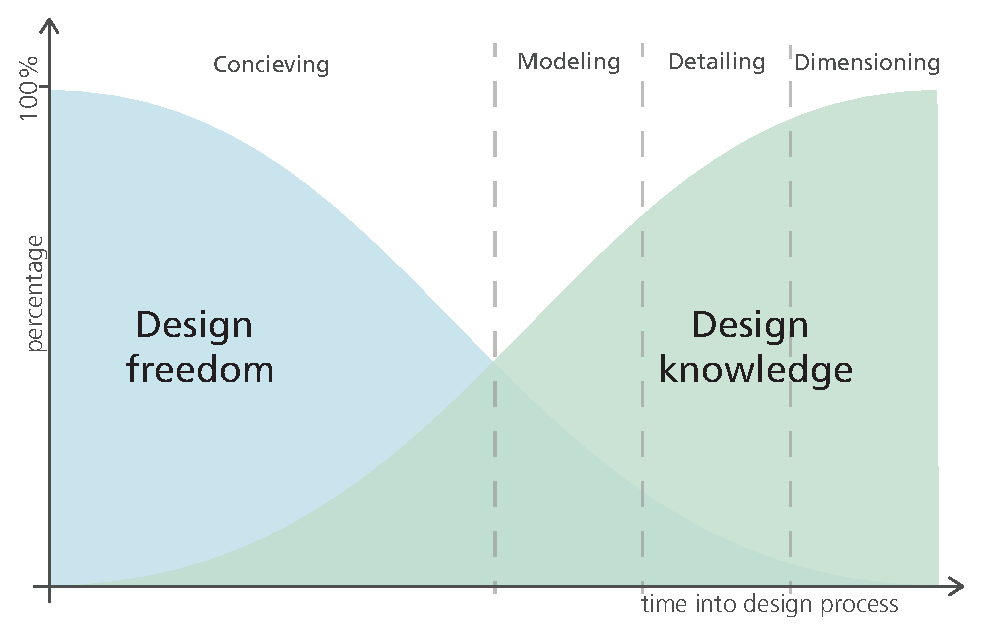
\includegraphics[width=350pt]{graphics/freedom-vs-knowledge.eps}
  \caption{Structural design process \cite{Mueller2014}}
  \label{fig:freedom-vs-knowledge}
\end{figure}

\section{Problem statement}
Many different geometric modeling tools are today available for architects. These geometric modeling tools have, since their introduction in the 1980s, grown increasingly sophisticated. They have also, together with the widespread perception of the benefits of technological innovation, created a more intimate relationship between technology and design. This relationship has resulted in parametric design and scripting methods that can generate complex shapes and forms \cite{sakamoto2008control}. The distinct separation found in practice where architect’s use geometric modeling tools and engineers use analysis tools further reinforces the architects role as \textit{form-giver }and the engineer as \textit{form-verifier }\cite{mueller2013integrated}. To move away from this separation, when the term \textit{designer }is used in this thesis it represents either an engineer or an architect. Instead of the current practice, it would be beneficial if the engineer and architect would collaborate as designers in the structural design process. This would allow physical demands to work as an inspiration, rather than as a constraint of what is possible, to find new well performing geometric forms. Where physical demands can for example be: structural performance, construction costs, operational energy needs, acoustics.

In the current practice the architect often conceives a design without involvement of the structural engineer. Hence, the importance of the conceptual design phase is often overlooked and structural aspects are often only considered in a late design stage \cite{schlaich2006challenges}. A contributing factor to this is that very few computational tools are available for conceptual design. 

\begin{figure}
  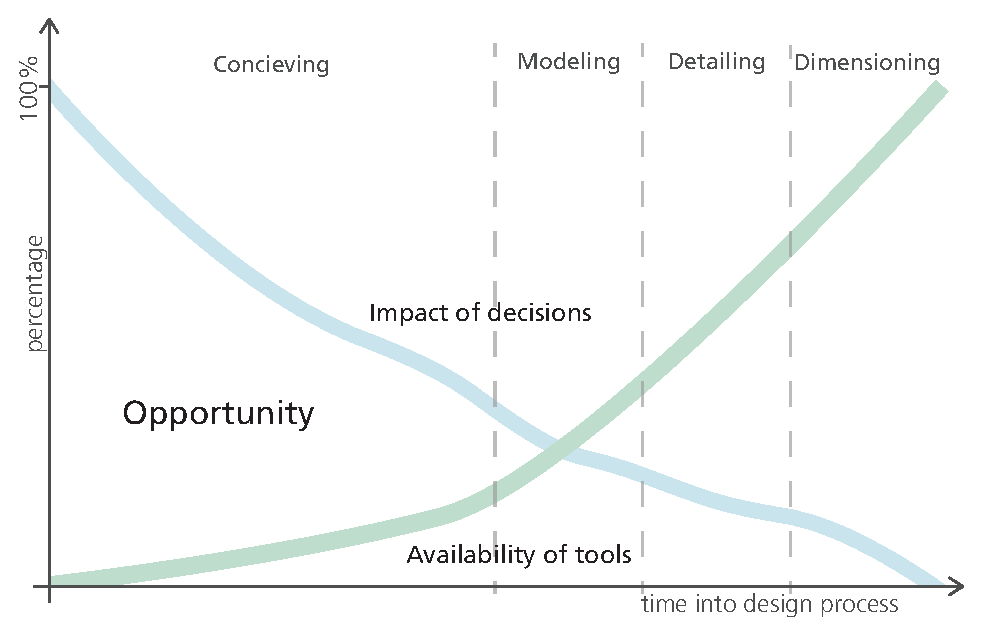
\includegraphics[width=350pt]{graphics/impact-tools.eps}
  \caption{Impact of decisions and availability of tools in the design process \cite{Hsu2000}}
  \label{fig:impact-tools}
\end{figure}


The challenge when developing such computational tools lies within the fuzzy nature of the problem, knowledge and constraints of the problem are imprecise and incomplete \cite{Hsu2000}.

Conventional advanced structural analysis software requires precise knowledge of the problem and is insufficiently agile to follow a designer’s iterative workflow. Conventional structural analysis software is developed for use in the late design stage, when the major design decisions have been made, as a tool for the engineer to verify the form. 

A subsequent problem with the traditional workflow, where the architect is the form-giver and the engineer is the from-verifier, can arise due to the availability of the a very detailed geometric model. It can be tempting for the engineer to directly perform a full analysis on the detailed geometry something which is possible with today’s structural analysis software. If instead the engineer starts with a simple mathematical model and then gradually increases the complexity - known as hierarchical modeling, see Figure \ref{fig:hiarchical-modelling} – the risk of fatal mistakes is decreased \cite{Bathe2006}. 

By starting with a simple mathematical model the engineer can focus on, and get a better understanding of, the overall structural behavior. Where the overall structural behavior is how stresses follow through the structure, what the magnitude of the stresses are in different structural members, etc. This information can be valuable when a more advanced mathematical model is used, to confirm the feasibility of the results. It has been shown that premature use of advanced structural analysis software negatively affects the conceptual understanding and the quality of the conceptual design \cite{Froderberg2014}.

In the present work, two similar computational conceptual design tools have been developed. The two applications make use of simple mathematical models, which enables structural modeling to be used earlier in the structural design process. The motivation for this is two-fold. It can give the designer valuable feedback on structural performance in the conceiving phase, when the impact of decision still is high. And it can also give the engineer valuable feedback on structural behavior before a more advanced model is used. 

\begin{figure}
  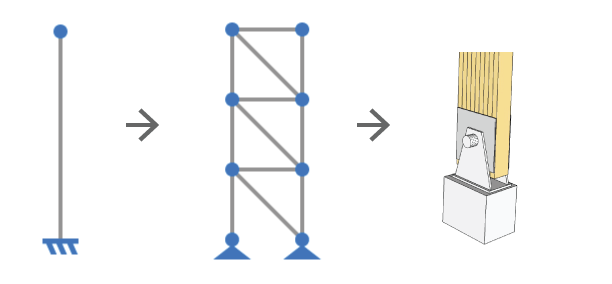
\includegraphics[width=270pt]{graphics/hiarchical-modelling.png}
  \caption{Hierarchical modeling}
  \label{fig:hiarchical-modelling}
\end{figure}

The type of design tool that is used to generate and represent ideas also affects the quality and quantity of early prototypes. It was shown in \cite{Haggman2015} that physical prototyping generated a higher quantity of prototypes, compared to using CAD or conventional sketching, under the same amount of time. The prototypes that were developed using physical prototyping were also perceived as more novel compared to the other prototypes. However, the prototypes that were perceived as more novel also tended to fare poorly on all other measureable qualities \cite{Haggman2015}. 

In the present work the prototypes are structural models. As computational models are used, a measurable performance can be computed and presented to the user in real-time. This can potentially can improve the quality of the structural models. The measureable performance and guidance in the present work put emphasis on the geometrical form of the structure as this has the greatest potential to improve the structural performance \cite{Mueller2014}. 

\subsection{Examples of well-executed conceptual structural design}
Structural demands can be integrated earlier in the design process by using them as inspiration of geometric forms instead of constraints of what is possible. Integrating structural demands earlier in the design process have the potential to reduce the amount of material needed, reduce environmental impact and lower costs for the project as a whole \cite{Mueller2014}. 

\begin{figure}
  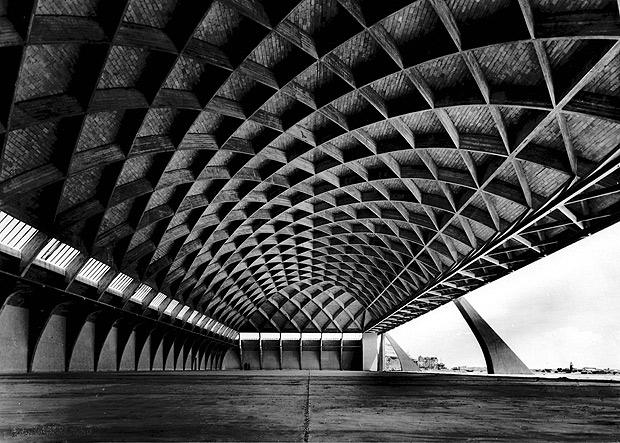
\includegraphics[width=350pt]{graphics/nervi.jpg}
  \caption{Pierre Luigi Nervi - Air hangar, built 1936}
  \label{fig:nervi}
\end{figure}

A good example of well-executed conceptual designs are the structures designed by the Italian architect-engineer Pierre Luigi Nervi, see example in Figure \ref{fig:nervi}. Despite the complexity of his structures his designs were often selected because they were the cheapest to build \cite{Addis2007}, as less material was needed for his designs compared to his competitors. This type of complex concrete structure is unfeasible when labor costs are high, due to the extensive formwork required \cite{Todisco2015}. However, This is something which could of course change in the future with the emergence of robots and digital manufacturing \cite{MadeByRobots}.

\textit{''His buildings are most remarkable for the clarity of their engineering. The power and grace of these extraordinary shapes and patterns stems directly from their structural logic, and are inseparable from it''} – Ada Louise about Pierre Luigi Nervi, 1960 \cite{Mueller2014}

The Shenzhen CITIC Financial Center, see Figure \ref{fig:Shenzen}, is a more recent example of well-executed integrated conceptual design. The perimeter frames are inspired by research on optimal discrete truss geometries to minimize the material needed \cite{Stromberg2012a}.

\begin{figure}
  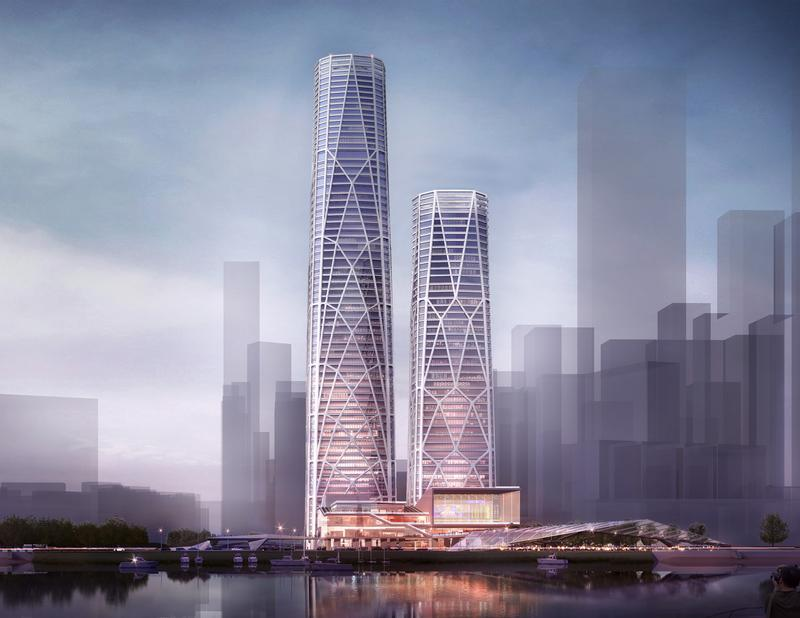
\includegraphics[width=350pt]{graphics/shenzen.jpg}
  \caption{Shenzen CITIC Financial Center, Lead Architectural Partner: Craig W. Hartman, Lead Structural Partner: Mark Sarkisian.  Rendering © Skidmore, Owings \& Merrill LLP, 2016}
  \label{fig:Shenzen}
\end{figure}

Designing Nervi’s air hangar in 1936 required a very thorough understanding of structural mechanics. He was at the time the only one, or one of very few engineers that was capable of successfully designing such a structure. The CITIC Financial center was also designed by a team distinguished designers. The difference between the two examples are that the latter used computer computations in the design process. 

\subsection{Computational design tools}
Computational design tools have the possibility make computer computations readily available in the design process, to help guide the designer towards well-performing solutions. Such tools have previously been developed and a review of existing tools and the methods that they implement are available in Chapter 3. These tools are developed to follow the designer’s iterative workflow, which the conventional structural analysis software lacks. 

Allowing these computational tools to follow the designer’s iterative workflow puts high demand on the user interface of the tools. Most of the existing computational design tools are developed for mouse and keyboard input. In the present work alternative input devices are explored, which allows for a more direct input. 

\section{Research methodology }
\subsection{Aim of research}
The long term goal with this research is to improve the conceptual design phase by integrating structural demands early in the design process. An improved conceptual design phase has the potential to improve the quality of structures in the built environment. These qualities can for example be: structural performance, construction costs, operational energy needs, acoustics.


\begin{itemize}  
\item To improve conceptual structural design by developing computational tools that bridge the gap between the design steps conceiving and modeling.
\item  To create intuitive conceptual structural design tools that allow the user to easily explore different design alternatives.
\item To improve the human-computer interaction for such tools though use of new, novel user input devices. 
\end{itemize}


\subsection{Research questions}
\begin{itemize}  
\item How can the human-computer interaction be improved in computational conceptual structural design tools?
\item  Which computational methods can be used to improve the conceptual design phase? 
\end{itemize}

\subsection{Research approach and limitations}
The present research is a multi-disciplinary work between structural mechanics, computer science and architecture. Methods from structural mechanics are used to provide the user with guidance and feedback. Developing user interfaces and employing programming techniques is a part of the computer science discipline. Studying conceptual design and finding geometrical forms are a part of architecture. The research is applied and any successful tools that this work results in could potentially be used in practice with few changes.

There are different research approaches to investigate how the conceptual structural design phase can be improved. In this work, it has only been investigated how new computational tools can improve the conceptual design phase. Project management, social aspects and culture is not considered in this work.

Many different computational methods exist that can be used for conceptual structural design. Some promising methods are presented in Chapter \ref{ch:Computational methods}, a selection of these methods have been used in the present work.

\subsection{Outline}
\textbf{Part I} is an introduction to the research area and also literature review of previous work in this field. This part is similar to, but an extension of, the introductory sections in the appended papers. \textbf{Chapter \ref{ch:Introduction}}, is an introduction to the research area, and motivates why this work is important. \textbf{Chapter \ref{ch:Human-computer interaction}} introduces human-computer interaction to the reader and introduces state of the art technology, such as new input devices. \textbf{Chapter \ref{ch:Computational methods}} , presents computational methods that can be applied to conceptual design. Different optimization methods, especially the genetic algorithm, are thoroughly introduced; as these methods will be used in future work. \textbf{Chapter \ref{ch:Literature review}} reviews existing conceptual structural design tools. In \textbf{Chapter \ref{ch:Integrating structural feedback}} requirements for integrating structural feedback in the conceptual design are presented, and a summary of the present work is presented. The publications that this work has resulted in are presented in \textbf{Chapter \ref{ch:Summary of appended papers}} and \textbf{Chapter \ref{ch:Results discussion}} summarizes the present work and the intellectual contributions. \textbf{Part II}  is appended publications.
